\documentclass{standalone}
\usepackage{tikz}
\usetikzlibrary{patterns, positioning}

\begin{document}
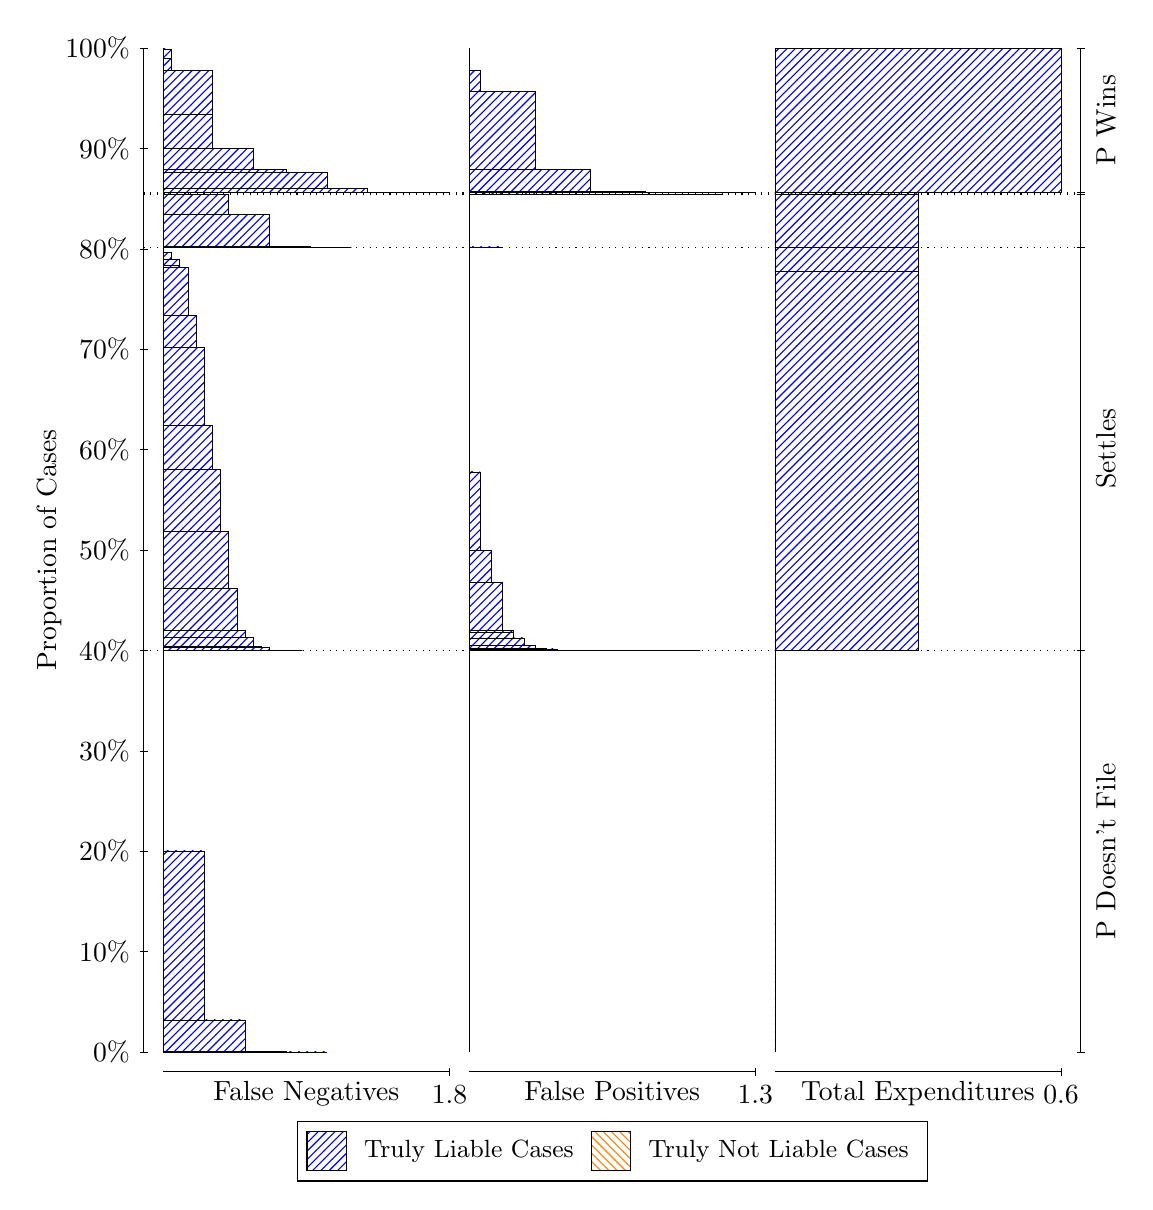
\begin{tikzpicture}
\draw[black, very thin] (1.5,1.75) -- (1.5,14.5);
\node[rotate=90, anchor=center] at (0.3, 8.125) {Proportion of Cases};
\draw[black, very thin] (1.45,1.75) -- (1.55,1.75);
\node[anchor=east] at (1.45, 1.75) {0\%};
\draw[black, very thin] (1.45,3.025) -- (1.55,3.025);
\node[anchor=east] at (1.45, 3.025) {10\%};
\draw[black, very thin] (1.45,4.3) -- (1.55,4.3);
\node[anchor=east] at (1.45, 4.3) {20\%};
\draw[black, very thin] (1.45,5.575) -- (1.55,5.575);
\node[anchor=east] at (1.45, 5.575) {30\%};
\draw[black, very thin] (1.45,6.85) -- (1.55,6.85);
\node[anchor=east] at (1.45, 6.85) {40\%};
\draw[black, very thin] (1.45,8.125) -- (1.55,8.125);
\node[anchor=east] at (1.45, 8.125) {50\%};
\draw[black, very thin] (1.45,9.4) -- (1.55,9.4);
\node[anchor=east] at (1.45, 9.4) {60\%};
\draw[black, very thin] (1.45,10.675) -- (1.55,10.675);
\node[anchor=east] at (1.45, 10.675) {70\%};
\draw[black, very thin] (1.45,11.95) -- (1.55,11.95);
\node[anchor=east] at (1.45, 11.95) {80\%};
\draw[black, very thin] (1.45,13.225) -- (1.55,13.225);
\node[anchor=east] at (1.45, 13.225) {90\%};
\draw[black, very thin] (1.45,14.5) -- (1.55,14.5);
\node[anchor=east] at (1.45, 14.5) {100\%};

\draw[black, very thin] (13.4,1.75) -- (13.4,14.5);
\draw[black, very thin] (13.35,1.75) -- (13.45,1.75);
\node[anchor=west] at (13.35, 1.75) {};
\draw[black, very thin] (13.35,6.8489) -- (13.45,6.8489);
\node[anchor=west] at (13.35, 6.8489) {};
\draw[black, very thin] (13.35,11.971) -- (13.45,11.971);
\node[anchor=west] at (13.35, 11.971) {};
\draw[black, very thin] (13.35,12.646) -- (13.45,12.646);
\node[anchor=west] at (13.35, 12.646) {};
\draw[black, very thin] (13.35,12.67) -- (13.45,12.67);
\node[anchor=west] at (13.35, 12.67) {};
\draw[black, very thin] (13.35,14.5) -- (13.45,14.5);
\node[anchor=west] at (13.35, 14.5) {};

\draw[black, very thin, pattern color=blue, pattern=north east lines] (1.75,1.75) rectangle (3.8262,1.75);
\draw[black, very thin, pattern color=blue, pattern=north east lines] (1.75,1.75) rectangle (3.3071,1.7534);
\draw[black, very thin, pattern color=blue, pattern=north east lines] (1.75,1.7534) rectangle (2.7881,2.158);
\draw[black, very thin, pattern color=blue, pattern=north east lines] (1.75,2.158) rectangle (2.269,4.3029);
\draw[black, very thin, pattern color=orange, pattern=north west lines] (1.75,4.3029) rectangle (1.75,4.3029);
\draw[black, very thin, pattern color=blue, pattern=north east lines] (1.75,4.3029) rectangle (1.75,6.8489);
\draw[black, very thin, pattern color=blue, pattern=north east lines] (1.75,6.8489) rectangle (3.5148,6.8489);
\draw[black, very thin, pattern color=blue, pattern=north east lines] (1.75,6.8489) rectangle (3.3071,6.849);
\draw[black, very thin, pattern color=blue, pattern=north east lines] (1.75,6.849) rectangle (3.0995,6.8846);
\draw[black, very thin, pattern color=blue, pattern=north east lines] (1.75,6.8846) rectangle (2.9957,6.898);
\draw[black, very thin, pattern color=blue, pattern=north east lines] (1.75,6.898) rectangle (2.8919,7.0201);
\draw[black, very thin, pattern color=blue, pattern=north east lines] (1.75,7.0201) rectangle (2.7881,7.102);
\draw[black, very thin, pattern color=blue, pattern=north east lines] (1.75,7.102) rectangle (2.6843,7.6406);
\draw[black, very thin, pattern color=blue, pattern=north east lines] (1.75,7.6406) rectangle (2.5805,8.3592);
\draw[black, very thin, pattern color=blue, pattern=north east lines] (1.75,8.3592) rectangle (2.4767,9.1532);
\draw[black, very thin, pattern color=blue, pattern=north east lines] (1.75,9.1532) rectangle (2.3729,9.7042);
\draw[black, very thin, pattern color=blue, pattern=north east lines] (1.75,9.7042) rectangle (2.269,10.699);
\draw[black, very thin, pattern color=blue, pattern=north east lines] (1.75,10.699) rectangle (2.1652,11.102);
\draw[black, very thin, pattern color=blue, pattern=north east lines] (1.75,11.102) rectangle (2.0614,11.714);
\draw[black, very thin, pattern color=blue, pattern=north east lines] (1.75,11.714) rectangle (1.9576,11.741);
\draw[black, very thin, pattern color=blue, pattern=north east lines] (1.75,11.741) rectangle (1.9576,11.811);
\draw[black, very thin, pattern color=blue, pattern=north east lines] (1.75,11.811) rectangle (1.8538,11.903);
\draw[black, very thin, pattern color=orange, pattern=north west lines] (1.75,11.903) rectangle (1.75,11.903);
\draw[black, very thin, pattern color=blue, pattern=north east lines] (1.75,11.903) rectangle (1.75,11.971);
\draw[black, very thin, pattern color=blue, pattern=north east lines] (1.75,11.971) rectangle (4.1376,11.971);
\draw[black, very thin, pattern color=blue, pattern=north east lines] (1.75,11.971) rectangle (3.6186,11.983);
\draw[black, very thin, pattern color=blue, pattern=north east lines] (1.75,11.983) rectangle (3.0995,12.391);
\draw[black, very thin, pattern color=blue, pattern=north east lines] (1.75,12.391) rectangle (2.5805,12.643);
\draw[black, very thin, pattern color=blue, pattern=north east lines] (1.75,12.643) rectangle (2.0614,12.646);
\draw[black, very thin, pattern color=orange, pattern=north west lines] (1.75,12.646) rectangle (1.75,12.646);
\draw[black, very thin, pattern color=blue, pattern=north east lines] (1.75,12.646) rectangle (2.0614,12.667);
\draw[black, very thin, pattern color=orange, pattern=north west lines] (1.75,12.667) rectangle (1.75,12.667);
\draw[black, very thin, pattern color=blue, pattern=north east lines] (1.75,12.667) rectangle (1.75,12.67);
\draw[black, very thin, pattern color=blue, pattern=north east lines] (1.75,12.67) rectangle (5.3833,12.67);
\draw[black, very thin, pattern color=blue, pattern=north east lines] (1.75,12.67) rectangle (4.8643,12.671);
\draw[black, very thin, pattern color=blue, pattern=north east lines] (1.75,12.671) rectangle (4.3452,12.715);
\draw[black, very thin, pattern color=blue, pattern=north east lines] (1.75,12.715) rectangle (3.93,12.715);
\draw[black, very thin, pattern color=blue, pattern=north east lines] (1.75,12.715) rectangle (3.8262,12.921);
\draw[black, very thin, pattern color=blue, pattern=north east lines] (1.75,12.921) rectangle (3.411,12.921);
\draw[black, very thin, pattern color=blue, pattern=north east lines] (1.75,12.921) rectangle (3.3071,12.955);
\draw[black, very thin, pattern color=blue, pattern=north east lines] (1.75,12.955) rectangle (2.8919,13.224);
\draw[black, very thin, pattern color=blue, pattern=north east lines] (1.75,13.224) rectangle (2.7881,13.224);
\draw[black, very thin, pattern color=blue, pattern=north east lines] (1.75,13.224) rectangle (2.3729,13.659);
\draw[black, very thin, pattern color=blue, pattern=north east lines] (1.75,13.659) rectangle (2.3729,14.215);
\draw[black, very thin, pattern color=blue, pattern=north east lines] (1.75,14.215) rectangle (2.269,14.215);
\draw[black, very thin, pattern color=blue, pattern=north east lines] (1.75,14.215) rectangle (1.8538,14.373);
\draw[black, very thin, pattern color=blue, pattern=north east lines] (1.75,14.373) rectangle (1.8538,14.489);
\draw[black, very thin, pattern color=orange, pattern=north west lines] (1.75,14.489) rectangle (1.75,14.489);
\draw[black, very thin, pattern color=blue, pattern=north east lines] (1.75,14.489) rectangle (1.75,14.5);
\draw[black, very thin, pattern color=orange, pattern=north west lines] (5.6333,1.75) rectangle (5.6333,1.75);
\draw[black, very thin, pattern color=blue, pattern=north east lines] (5.6333,1.75) rectangle (5.6333,6.8489);
\draw[black, very thin, pattern color=orange, pattern=north west lines] (5.6333,6.8489) rectangle (8.5679,6.8489);
\draw[black, very thin, pattern color=blue, pattern=north east lines] (5.6333,6.8489) rectangle (8.5679,6.8489);
\draw[black, very thin, pattern color=orange, pattern=north west lines] (5.6333,6.8489) rectangle (8.2885,6.8489);
\draw[black, very thin, pattern color=blue, pattern=north east lines] (5.6333,6.8489) rectangle (8.2885,6.8489);
\draw[black, very thin, pattern color=orange, pattern=north west lines] (5.6333,6.8489) rectangle (8.009,6.8489);
\draw[black, very thin, pattern color=blue, pattern=north east lines] (5.6333,6.8489) rectangle (8.009,6.8489);
\draw[black, very thin, pattern color=blue, pattern=north east lines] (5.6333,6.8489) rectangle (7.8692,6.8489);
\draw[black, very thin, pattern color=orange, pattern=north west lines] (5.6333,6.8489) rectangle (7.7295,6.8489);
\draw[black, very thin, pattern color=blue, pattern=north east lines] (5.6333,6.8489) rectangle (7.7295,6.8489);
\draw[black, very thin, pattern color=blue, pattern=north east lines] (5.6333,6.8489) rectangle (7.5897,6.8489);
\draw[black, very thin, pattern color=orange, pattern=north west lines] (5.6333,6.8489) rectangle (7.45,6.8489);
\draw[black, very thin, pattern color=blue, pattern=north east lines] (5.6333,6.8489) rectangle (7.45,6.8489);
\draw[black, very thin, pattern color=blue, pattern=north east lines] (5.6333,6.8489) rectangle (7.3103,6.8489);
\draw[black, very thin, pattern color=orange, pattern=north west lines] (5.6333,6.8489) rectangle (7.1705,6.8489);
\draw[black, very thin, pattern color=blue, pattern=north east lines] (5.6333,6.8489) rectangle (7.1705,6.8489);
\draw[black, very thin, pattern color=blue, pattern=north east lines] (5.6333,6.8489) rectangle (7.0308,6.849);
\draw[black, very thin, pattern color=blue, pattern=north east lines] (5.6333,6.849) rectangle (6.891,6.8491);
\draw[black, very thin, pattern color=orange, pattern=north west lines] (5.6333,6.8491) rectangle (6.891,6.8491);
\draw[black, very thin, pattern color=blue, pattern=north east lines] (5.6333,6.8491) rectangle (6.891,6.8491);
\draw[black, very thin, pattern color=blue, pattern=north east lines] (5.6333,6.8491) rectangle (6.7513,6.8681);
\draw[black, very thin, pattern color=blue, pattern=north east lines] (5.6333,6.8681) rectangle (6.6115,6.8781);
\draw[black, very thin, pattern color=blue, pattern=north east lines] (5.6333,6.8781) rectangle (6.4718,6.9177);
\draw[black, very thin, pattern color=blue, pattern=north east lines] (5.6333,6.9177) rectangle (6.3321,7.0089);
\draw[black, very thin, pattern color=blue, pattern=north east lines] (5.6333,7.0089) rectangle (6.1923,7.0798);
\draw[black, very thin, pattern color=blue, pattern=north east lines] (5.6333,7.0798) rectangle (6.1923,7.1068);
\draw[black, very thin, pattern color=blue, pattern=north east lines] (5.6333,7.1068) rectangle (6.0526,7.7183);
\draw[black, very thin, pattern color=blue, pattern=north east lines] (5.6333,7.7183) rectangle (5.9128,8.1208);
\draw[black, very thin, pattern color=blue, pattern=north east lines] (5.6333,8.1208) rectangle (5.7731,9.1161);
\draw[black, very thin, pattern color=blue, pattern=north east lines] (5.6333,9.1161) rectangle (5.6333,11.971);
\draw[black, very thin, pattern color=orange, pattern=north west lines] (5.6333,11.971) rectangle (6.0526,11.971);
\draw[black, very thin, pattern color=blue, pattern=north east lines] (5.6333,11.971) rectangle (6.0526,11.974);
\draw[black, very thin, pattern color=blue, pattern=north east lines] (5.6333,11.974) rectangle (5.6333,12.646);
\draw[black, very thin, pattern color=orange, pattern=north west lines] (5.6333,12.646) rectangle (8.8474,12.646);
\draw[black, very thin, pattern color=blue, pattern=north east lines] (5.6333,12.646) rectangle (8.8474,12.646);
\draw[black, very thin, pattern color=blue, pattern=north east lines] (5.6333,12.646) rectangle (8.1487,12.646);
\draw[black, very thin, pattern color=blue, pattern=north east lines] (5.6333,12.646) rectangle (7.45,12.646);
\draw[black, very thin, pattern color=blue, pattern=north east lines] (5.6333,12.646) rectangle (6.7513,12.649);
\draw[black, very thin, pattern color=blue, pattern=north east lines] (5.6333,12.649) rectangle (6.0526,12.67);
\draw[black, very thin, pattern color=orange, pattern=north west lines] (5.6333,12.67) rectangle (9.2667,12.67);
\draw[black, very thin, pattern color=blue, pattern=north east lines] (5.6333,12.67) rectangle (9.2667,12.67);
\draw[black, very thin, pattern color=orange, pattern=north west lines] (5.6333,12.67) rectangle (8.5679,12.67);
\draw[black, very thin, pattern color=blue, pattern=north east lines] (5.6333,12.67) rectangle (8.5679,12.67);
\draw[black, very thin, pattern color=orange, pattern=north west lines] (5.6333,12.67) rectangle (7.8692,12.67);
\draw[black, very thin, pattern color=blue, pattern=north east lines] (5.6333,12.67) rectangle (7.8692,12.681);
\draw[black, very thin, pattern color=orange, pattern=north west lines] (5.6333,12.681) rectangle (7.1705,12.681);
\draw[black, very thin, pattern color=blue, pattern=north east lines] (5.6333,12.681) rectangle (7.1705,12.955);
\draw[black, very thin, pattern color=orange, pattern=north west lines] (5.6333,12.955) rectangle (6.6115,12.955);
\draw[black, very thin, pattern color=blue, pattern=north east lines] (5.6333,12.955) rectangle (6.6115,12.955);
\draw[black, very thin, pattern color=blue, pattern=north east lines] (5.6333,12.955) rectangle (6.4718,13.946);
\draw[black, very thin, pattern color=orange, pattern=north west lines] (5.6333,13.946) rectangle (5.9128,13.946);
\draw[black, very thin, pattern color=blue, pattern=north east lines] (5.6333,13.946) rectangle (5.9128,13.946);
\draw[black, very thin, pattern color=blue, pattern=north east lines] (5.6333,13.946) rectangle (5.7731,14.215);
\draw[black, very thin, pattern color=orange, pattern=north west lines] (5.6333,14.215) rectangle (5.6333,14.215);
\draw[black, very thin, pattern color=blue, pattern=north east lines] (5.6333,14.215) rectangle (5.6333,14.5);
\draw[black, very thin, pattern color=orange, pattern=north west lines] (9.5167,1.75) rectangle (9.5167,1.75);
\draw[black, very thin, pattern color=blue, pattern=north east lines] (9.5167,1.75) rectangle (9.5167,6.8489);
\draw[black, very thin, pattern color=orange, pattern=north west lines] (9.5167,6.8489) rectangle (11.333,6.8489);
\draw[black, very thin, pattern color=blue, pattern=north east lines] (9.5167,6.8489) rectangle (11.333,11.668);
\draw[black, very thin, pattern color=orange, pattern=north west lines] (9.5167,11.668) rectangle (11.333,11.668);
\draw[black, very thin, pattern color=blue, pattern=north east lines] (9.5167,11.668) rectangle (11.333,11.971);
\draw[black, very thin, pattern color=orange, pattern=north west lines] (9.5167,11.971) rectangle (11.333,11.971);
\draw[black, very thin, pattern color=blue, pattern=north east lines] (9.5167,11.971) rectangle (11.333,12.646);
\draw[black, very thin, pattern color=orange, pattern=north west lines] (9.5167,12.646) rectangle (11.333,12.646);
\draw[black, very thin, pattern color=blue, pattern=north east lines] (9.5167,12.646) rectangle (11.333,12.67);
\draw[black, very thin, pattern color=orange, pattern=north west lines] (9.5167,12.67) rectangle (13.15,12.67);
\draw[black, very thin, pattern color=blue, pattern=north east lines] (9.5167,12.67) rectangle (13.15,14.5);
\draw[black, dotted] (1.5,6.8489) -- (13.4,6.8489);
\draw[black, dotted] (1.5,11.971) -- (13.4,11.971);
\draw[black, dotted] (1.5,12.646) -- (13.4,12.646);
\draw[black, dotted] (1.5,12.67) -- (13.4,12.67);
\draw[black, very thin] (1.75,1.5) -- (5.3833,1.5);
\node[anchor=north] at (3.5667, 1.5) {False Negatives};
\draw[black, very thin] (5.3833,1.45) -- (5.3833,1.55);
\node[anchor=north] at (5.3833, 1.45) {1.8};

\draw[black, very thin] (5.6333,1.5) -- (9.2667,1.5);
\node[anchor=north] at (7.45, 1.5) {False Positives};
\draw[black, very thin] (9.2667,1.45) -- (9.2667,1.55);
\node[anchor=north] at (9.2667, 1.45) {1.3};

\draw[black, very thin] (9.5167,1.5) -- (13.15,1.5);
\node[anchor=north] at (11.333, 1.5) {Total Expenditures};
\draw[black, very thin] (13.15,1.45) -- (13.15,1.55);
\node[anchor=north] at (13.15, 1.45) {0.6};

\node[black, centered, rotate=90] at (13.72, 4.2994) {P Doesn't File};
\node[black, centered, rotate=90] at (13.72, 9.4101) {Settles};


\node[black, centered, rotate=90] at (13.72, 13.585) {P Wins};

\draw (7.449999999999999,1.5) node[draw=none] (baseCoordinate) {};
\begin{scope}[align=center]
        \matrix[scale=0.5, draw=black, below=0.5cm of baseCoordinate, nodes={draw}, column sep=0.1cm]{
            \node[rectangle, draw, minimum width=0.5cm, minimum height=0.5cm, pattern=north east lines, pattern color=blue] {}; &
            \node[draw=none, font=\small] (B) {Truly Liable Cases}; &
            \node[rectangle, draw, minimum width=0.5cm, minimum height=0.5cm, pattern=north west lines, pattern color=orange] {}; &
            \node[draw=none, font=\small] (B) {Truly Not Liable Cases}; \\
            };
\end{scope}

\end{tikzpicture}
\end{document}